

\documentclass[a4paper,12pt]{article}
\usepackage{ucs} 
\usepackage[utf8x]{inputenc}
\usepackage[ngerman]{babel} 
\usepackage[T1]{fontenc} 
\usepackage[pdftex]{graphicx}   
\usepackage{listings} % for sourcecode
\usepackage{bera}
\usepackage{showexpl}
\usepackage{xcolor}
\usepackage{textcomp}

\def\listingsfont{\ttfamily}

\begin{document}
\lstset{language=C++,
                %basicstyle=\smallest\ttfamily,
                keywordstyle=\color{blue}\ttfamily,
                stringstyle=\color{red}\ttfamily,
                commentstyle=\color{green}\ttfamily,
                morecomment=[l][\color{magenta}]{\#},
								breaklines=true,}

%% Basierend auf einer TeXnicCenter-Vorlage von Tino Weinkauf.
%%%%%%%%%%%%%%%%%%%%%%%%%%%%%%%%%%%%%%%%%%%%%%%%%%%%%%%%%%%%%%

%%%%%%%%%%%%%%%%%%%%%%%%%%%%%%%%%%%%%%%%%%%%%%%%%%%%%%%%%%%%%
%% Deckblatt
%%%%%%%%%%%%%%%%%%%%%%%%%%%%%%%%%%%%%%%%%%%%%%%%%%%%%%%%%%%%%
%%
%% ACHTUNG: Sie ben�tigen ein Hauptdokument, um diese Datei
%%          benutzen zu k�nnen. Verwenden Sie im Hauptdokument
%%          den Befehl "\input{dateiname}", um diese
%%          Datei einzubinden.
%%

\begin{titlepage}

\begin{center}

%\vspace*{1cm}
\Large
\textsc{Graphische Datenverarbeitung}\\

\vspace{4cm}

\textsc{OpenGL Example}\\

\vspace{4cm}

\small

\textsc{Dokumentation\\[0.5\baselineskip]
von\\[0.5\baselineskip]
Daniel Bulla}\\

\large

\vspace{4cm}
\textsc{18. November 2013}\\ %%\today Datum der Abgabe - am besten selbst reinschreiben.

\vspace{1cm}
\textsc{Betreuer:\\
Prof. Dipl.-Inf. Ingrid Scholl}\\

\vspace{0.5cm}
\textsc{Fachhochschule Aachen\\
Fachbereich Informatik\\
Institut fu"r Graphische Datenverarbeitung}\\

\end{center}

\end{titlepage}

\section{Einleitung}
Diese Dokumentation bietet zusätzliche Information zum (kommentierten) Quellcode und zur Funktionsweise der Software "`ShaderTestScene"'.
Die Software kann unter https://github.com/epxzz/QtOpenGLTutorial heruntergeladen werden.
Das Projekt ist im Rahmen meiner Tätig als Hilfswerkstudent am Insititut für entstanden.
Bei der Erstellung von OpenGL-Anwendungen gibt es einige Pitfalls, welche hier beleuchtet werden. Grade durch die Verwenundung der neuen OpenGL Versionen ist die Lernkurve nicht mehr so steil wir bei älteren Versionen, welche die "`fixed function pipeline"' verwenden. Bei der Lösungssuche im Internet und Büchern ist umbedingt darauf zu achten, keine veralteten OpenGL versionen zu verwenden. Dabei hilft uns in diesem Beispiel die minimale Kapselung der OpenGL API durch Qt.
Für die meisten Leser sind natürlich die direkten Aufrufe der OpenGL-API von Interesse. Dennoch bietet uns Qt wichtige Vorteile die es uns ermöglichen, uns direkt die interessanten Aspekte der OpenGL-Programmierung zu konzentrieren. Auch wenn wir die Abhängigkeit von Qt entfernen wollen, so kämen Abhängigkeiten an eine Bibliothek für "`extension loading"'(TODO: Fußnote: http://rastergrid.com/blog/2010/03/sad-facts-about-opengl-extension-libraries/) hinzu, eine Matrix/Vector-Mathematik und Eingabegeräte (TODO: Fußnote, natürlich können die Funktionen auch ohne Bibliothek implementiert werden). Im Gegensatz zu DirectX, wo der Einstieg durch Microsoft sehr leicht gestaltet wird, kann der Einstieg in OpenGL beliebig schwierig sein.
Qt macht den Einstieg in OpenGL ähnlich einfach wie den Einstieg in DirectX. Qt ist in Module aufgeteilt - QtGui muss nicht zwangsweise verwendet werden. Andernfalls lässt sich die Qt Gui in eigenen 3D Renderings verwenden - den Qt kann intern OpenGL als Renderer verwenden.
\section{Installation}
Gezeigt wird ein Systemsetup, so dass Qt mit Visual Studio verwendet werden kann. Zum Beispiel für die Gui Programmierung kann während der Entwicklung gleichzeitig der QtCreator verwendet werden. Visual Studio kann durch das Plugin "`Nsight"' von Nvidia das Debuggen enorm vereinfachen. Es ist möglich Breakpoints in Shader zu setzen. Es kann ein einzelner Pixel für einen Fragmentshader ausgewählt werden, für den der zugehörige Shader gedebuggt werden soll. Profiling der (Nvidia-)Grafikkarte wird ebenfalls möglich.
In Verbindung mit einem QtQuickView war Nsight zum Zeitpunkt des Schreiben noch nicht verwendbar. Da Qt und Nsight (für OpenGL) sehr neue Entwicklungen sind, gehe ich davon aus, dass dieses Problem in den nächsten Monaten durch neue Versionen gelöst wurde. (TODO: Fußnote, link Nvidia forum. glVertexAttribPointer client side Vertex arrays)
\subsection{Vorraussetzungen}
\begin{enumerate}
\item
Visual Studio 2012. Die Express Version unterstützt nicht das Nsight- und Qt-AddIn. Verwendung von Qt sollte trotzdem möglich sein.
\item
Qt 5.1.1 for Windows 64-bit (VS 2012, OpenGL). VS2012 bedeutet, dass der Visual Studio Compiler verwendet wird. (TODO: Link: http://qt-project.org/downloads)
\item
Visual Studio Add-in 1.2.2 for Qt5. Das AddIn funktioniert nicht mit der Express Version. Es bietet uns die einfach Möglichkeit, Qt-Projekte aus Visual Studio zu erzeugen und Projekteinstellungen direkt in VS vorzunehmen.
\item
Optional: NVIDIA Nsight Visual Studio Edition. Das AddIn ist ebenfalls für Eclipse verfügbar. Für den Download ist ein Nvidia Developer Account nötig. (TODO:Link) https://developer.nvidia.com/nvidia-nsight-visual-studio-edition
\item
Optional: passender Treiber für Nsight. Evtl. muss ein Beta-Treiber für die fehlerfreie Verwendung von Nsight installiert sein. Falls es zu scheinbar unpassenden Fehlermeldungen beim Debuggen durch Nsight kommt, kann dies die Ursache sein.
\end{enumerate}
\subsection{Installation}
Die Installation der Komponenten ist Selbsterklärend.
Bei der Installation von Qt wird ein Unterordner "`(Installationsordner)\\Qt5.1.1\\5.1.1\\msvc2012\_64\_opengl"' angelegt. Dieser enth"a'lt die zu verwendende Qt Version.
\subsection{Projekt Einstellungen}
Beim Erstellen oder importieren eines Projektes müssen zwei Anpassungen gemacht werden.
Als Platform muss x64 ausgewählt werden. (TODO: Bild)
Markieren Sie die Projektmappe im Projektmappen-Explorer und wählen Sie "`Projektmappen Qt Version ändern"'. Wählen Sie "`msvc2012\_64\_opengl"' und bestätigen Sie den Dialog. Das Projekt sollte nun kompilieren. Bei importierten Projekten kann es nötig sein, weitere Qt-Module zum Projekt hinzuzufügen.
TODO:Path?
\subsection{Visual Studio 2012 Nvidia Nsight Plugin}
\section{Überblick}
\subsection{Verwendung}
\begin{figure}
	\centering
		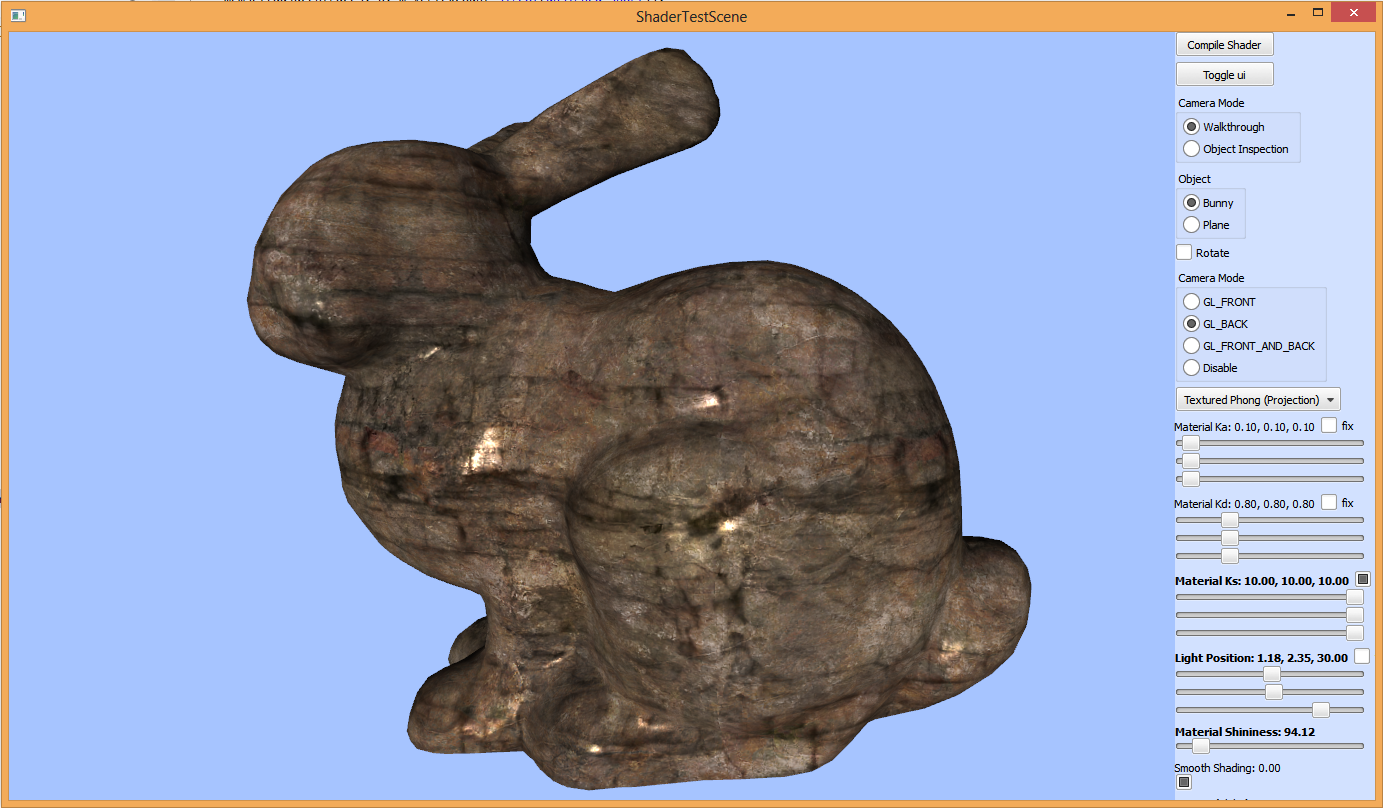
\includegraphics[width=\textwidth,height=\textheight,keepaspectratio]{Bilder/SpecularMap.png}
	\caption{Die Anwendung}
	\label{fig:Interface}
\end{figure}
Auf der rechten Seite sind alle Einstellungen zu finden.
\begin{enumerate}
\item
Camera Mode: Zwei Modi stehen zur Verfügung. Im Modus Walkthrough kann die Kamera mit den Tasten W,A,S,D gesteuert werden. Wird zu Object Inspection umgeschaltet, wird der aktuell anfokusierte Punkt als rotationspunkt verwendet.
\item
Object: Es kann zwischen zwei Objekten gewählt werden. Vorsicht: Das Modell "`Plane"' enthält sehr viel weniger Knoten als "`Bunny"'. Beim Wechsel der Objekte sollte kein zu hoher Tesselation-Faktor gewählt sein.
\item
Rotate: Verändert die "`ModelMatrix"'. Soll sich z.B. das Licht nicht mit drehen, darf es nicht mit der ModelMatrix transformiert werden.
\item
Cull Mode: Überspringt die Füllung eines Polygons von der Angegebenen Seite. Bei Lichtundurchlässigen Objekten können Rückseitige Polygone verworfen werden, um die Performance zu erhöhen. Die Richtung eines Polygons wird dabei technisch nicht über eine Normale, sondern über die Anordnung der Knoten in Bildkoordinaten bestimmt (Im Uhrzeigersinn oder dagegen).
\item
GL\_TEXTURE\_MIN\_FILTER: Bestimmt das Verhalten bei des texture-mapping, falls ein texel kleiner ist als die Fläche, auf die er gemappt wird (meist Pixel). Ein Unterschied ist zu sehen, wenn man weit heraus zoomt.
\item
GL\_TEXTURE\_MIN\_FILTER: Bestimmt das Verhalten bei des texture-mapping, falls ein texel größer ist als die Fläche, auf die er gemappt wird. Ein Unterschied ist zu sehen, wenn man nah heran zoomt.
\item Anisotropy: Verbessert Texturfilter bei hohen Betrachtungswinkeln. Ein Unterschied ist am besten am Model "`Plane"' zu sehen, wenn sich die Kamera nah an der Oberfläche befindet.
\item Shader: Eine Auswahl an Shadern. Die Auswahl an Shadern ist in der Datei "`./ui/overlay.qml"' definiert. Durch drücken von "`R"' wird die Datei neu eingelesen. So können neue Shader hinzugefügt werden, ohne das Prgamm neu zu kompilieren oder neu zu starten. Die Shader selbst befinden sich im Ordner "`./resources./shaders"'.
\end{enumerate}
\subsubsection{Shader Uniforms}
Die Folgenden Parameter können von Shadern verwendet werden. Nicht alle Slider werden in jedem Shader berücksichtigt. Der Shader "`Simple Phong"' soll einen einfachen Einstieg in die Programmierung bieten. Er unterstützt dafür nicht die zusätzliche Wireframe-Ansicht oder Tesselation.
\begin{enumerate}
\item Material Ka: Umgebungsbeleuchtung, unabhängig von Betrachtungswinkel und Lichtquelle. Vergleichbar mit dem Sonnenlicht, welches durch die Atmosphäre gleichmäßig verteilt wird.
\item Material Kd: Reaktion der Oberfläche auf diffuses Licht. Abhängig vom Oberflächenwinkel zur Lichtquelle.
\item Material Ks: Lichtreflektion (specular lighting). Abhängig von Betrachtungswinkel. Die vorhandenen Shader nutzen den Wert für ein einfaches Model zur Simulation der Reflektion einer Punkt-Lichtquelle.
\item Use Specular Map: Der Shader verwendet eine Textur, welche die Glanzkraft der Oberfläche kodiert. Bei einem Steinboden reflektieren die Steine so mehr als ihr Untergrund.
\item Specular Map Factor: Intensität der Specular Map. Negative Werte invertieren die Specular Map. Z.B. bei Nässe, reflektieren alle Stellen einer Oberfläche.
\item Light Position: x/y/z-Koordinaten des Lichts.
\item Material Shininess (log): Beeinflusst die Größe des Reflektionspunkt. Logarithmische Skala.
\item Texture Scale: Verändert die Größe der Textur.
\item Smooth Shading: Schaltet Gouraud Shading ein und aus. Weiche Normalen für Knoten können nicht durch Shader berechnet werden. Per-face-normale hingegen schon. Wird Smooth-Shading abgeschaltet, so berechnet ein Geometry-Shader die Normalen "`per face"'/für flat-shading. 
\item Opacity: Deckkraft/Transparenz. In Verbindung mit Cull Mode interessant.
\item Explode: Einige Beispielshader unterstützen diese Einstellung. Knoten werden um diesen Faktor entlang der Normalen nach außen verschoben.
\item Scale Faces on Explode: Für die Verschiebung wird entweder die per-vertex- oder die per-face-Normale verwendet.
\item Wireframe Einstellungen: Schaltet zusätzlich die Darstellung des Drahtgittermodells ein. Die Implementierung verwendet keine Linien-primitve. Dadurch wird z.B. culling unterstützt.
\item Fur Levels: Der Fur-Shader nutzt die Einstellung um volumenartiges Fell zu erzeugen. Dabei wird das Modell öffter nacheinander gezeichnet und dabei die "`explode"'-Funktion verwendet. Für alle anderen Shader sollte die Einstellung umbedingt auf 1 stehen, da sonst öfter hintereinander das selbe Rendering berechnet wird und sich selbst immer wieder überschreibt.
\item Tess Level Inner: Unterteilung eines Patches (in dieser Anwendung immer Dreiecke) in kleinere Primitive. Die äußere Form des Patches wird nicht verändert. Somit entsteht z.B. zwischen zwei Dreiecken mit unterschiedlichen inneren Tesselation-Leveln keine Überlappungen oder Löcher.
\item Tess Level Outer: Bestimmt in wieviele Teile die Kanten eine Patches unterteilt werden.
\item Tess Scale: wird von dem Shader als Höhe interpretiert. Knoten, auf deren Position eine die Height-Map-Texture einen hohen Wert kodiert hat, werden um diesen Wert nach außen verschoben.
\item Bump normal influence: Beeinflusst die Umrechnung der kodierten Normalen aus einer Textur in den Tangentenraum.
\item Mr. Wiggle Einstellungen: Erzeugt eine Animation. Entlang der x-Achse entstehen Wellen, die Knoten entlang ihrer Normalen nach außen drücken. Auch die Normale der Knoten wird dabei aktualisiert.
\end{enumerate}
\subsection{Softwareentwurf}
\begin{figure}
	\centering
		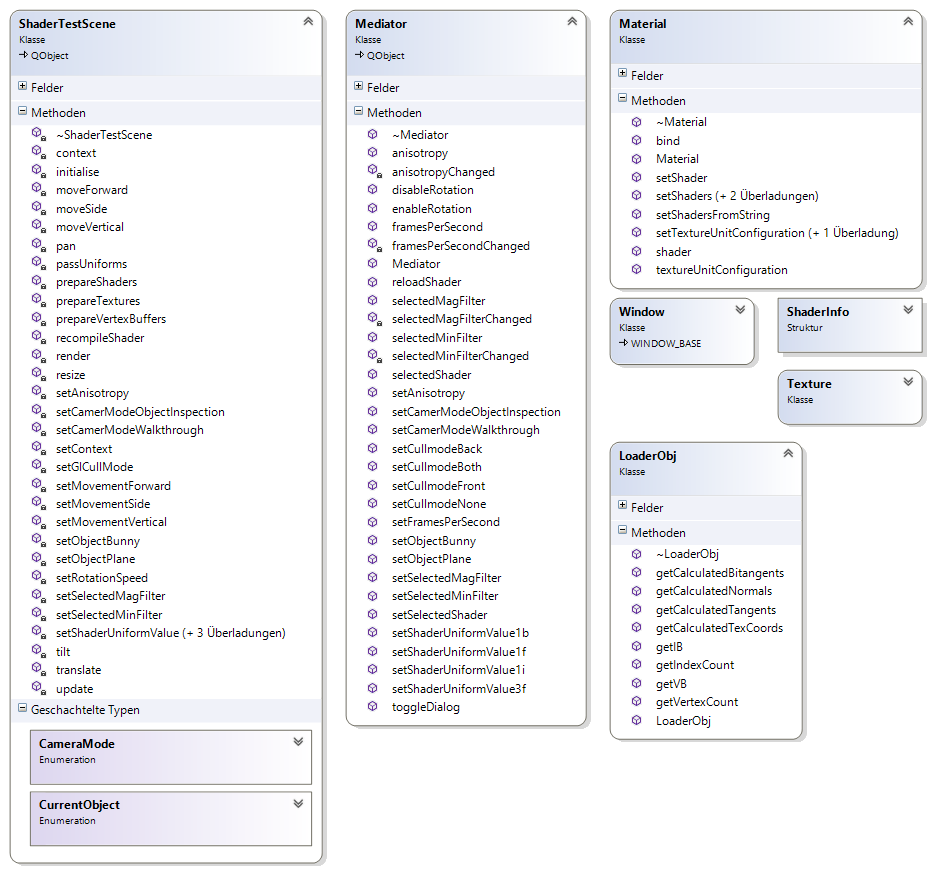
\includegraphics[width=\textwidth,height=\textheight,keepaspectratio]{Bilder/Klassendiagramm.png}
	\label{fig:Klassendiagramm}
\end{figure}
Das Beispielprojekt soll einen möglichst einfachen Einstieg in die OpenGL-Entwicklung mit C++ bieten. Gleichzeitig soll es einfach sein, neue Shader zu erstellen und sie mit der Benutzeroberfläche zu verbinden. Die Klasse ShaderTestScene enthält die nötige Funktionalität um eine 3D-Szene darzustellen. Sie enthält einige getter und setter, mit der sich die Klasse von außen steuern lässt. Die Klasse Mediator dient als Verbindung der Benutzeroberfläche mit ShaderTestScene, Mediator verwendet die getter und setter. Die Benutzeroberfläche selbst ist in QML geschrieben. Die Qml-Datei enthält auch die Pfäde zu den Shaderdateien, die zur Auswahl stehen. Auch die Werte, die über Schieberegler in der Anwendung zu sehen sind, werden dort definiert.

\section{OpenGL Calls}
Die Aufrufe sind durch Qt gekapselt. Es sollte einfach möglich sein, die entsprechenden OpenGL Funktionen zu finden.
\subsection{Initialisierung}
\subsubsection{Screen}
Als erster Schritt wird in der Klasse "`Window"' der das Bildschirmformat bestimmt. Wir "`leihen"' uns den OpenGL Context eines QQuickWindows. Trotzdem haben wir durch die Funktion "`QQuickWindow::setFormat(QSurfaceFormat format)"' die volle Kontrolle über die Initialisierung. 
In der Beispielanwenung gibt es zirkuläre Abhängigkeit bei der Initilisierung. Die Benutzeroberfläche versucht (Uniform-)Variablen zu setzen. Zu diesem Zeitpunkt wurden Shader noch nicht initialisiert. Der Shader wird in der Benutzeroberfläche gewählt und kann daher erst nach der Benutzeroberfläche erzeugt werden. Aus diesem Grund werden Variablen für Shader in mehreren HashMaps zwischengespeichert. Diesem Mechanismus sollte nicht zu viel Aufmerksamkeit geschenkt werden, er ist nicht fundamental wichtig.

\paragraph{Logging}
OpenGL hat einen internen Zustand. In großen Programmen muss mit allen Mitteln versucht werden, die Übersicht über diesen Zustand zu behalten. Es kann relativ einfach passieren, dass unbeabsichtigt unerlaubte Zustände entstehen. Fehlermeldungen treten dann vielleicht erst bei einem folgenden OpenGL-Aufruf auf und man sucht dein Fehler an einer falschen Stelle. Nach jedem gl*-Aufruf sollte die Methode glGetError für eine Fehlerbehandlung verwendet werden. Dies macht den Code unleserlich und es wird seid langem diskutiert, andere Mechanismen für die Fehlersuche durch OpenGL anzubieten (TODO: REF http://www.kdab.com/opengl-in-qt-5-1-part-4/).
QOpenGLDebugLogger erledigt Debugging sauberer.
\begin{lstlisting}[frame=single, columns=fullflexible]
if(m_logger.initialize()) {
 connect( &m_logger, SIGNAL(messageLogged(QOpenGLDebugMessage )),
  this, SLOT(onMessageLogged(QOpenGLDebugMessage )),
  Qt::DirectConnection);
 m_logger.startLogging(QOpenGLDebugLogger::SynchronousLogging);
 m_logger.enableMessages();
}
\end{lstlisting}
\subsubsection{Buffer}
In früheren Versionen von OpenGL gab es den "`Immediate mode"'. Dabei waren keine Puffer notwendig. Z.B. mit glVertex(x, y, z) konnten der Grafikkarte die Koordinaten für einen Punkt übergeben werden. Drei Aufrufe davor führten zu einem Dreieck und mehrere dann zu Objekten. Bei diesem Vorgehen werden Grafikkarte und CPU stark beansprucht. Deshalb ist dieses Vorgehen seit OpenGL 3.x entfernt worden.

Für jedes zu rendernde Objekt werden nun Puffer benötigt. Der gesammte Puffer kann dann an die Grafikkarte gesendet werden. Später teilen wir dem Programm/der Grafikkate mit, wie die einzelnen Puffer zu interpretieren sind. Seit der Abschaffung der fixed-function-Pipeline, muss die Grafikkarte jedoch nicht mehr wissen, ob es sich bei den Pufferinhalten um Positions- oder Farbwerte handelt. Wir werden die Pufferinhalte an Shadervariablen mappen.
Im Beispielprogramm sollen die Knoten der Objekte folgende Eigenschaften haben. Für jede Eigenschaft reservieren wir einen Puffer:
\begin{enumerate}
\item
Position - Koordinaten eines Punktes im Raum
\item
Normale - normalisierter Vector, welcher senkrecht auf der Oberfläche des Knotens steht.
\item
Tangente - normalisierter Vector, welcher in der Ebene liegt, die die Oberfläche des Knotens bildet. Zeigt in Richtung der Änderung der ersten Texturkoordinate.
\item
Bitangente - normalisierter Vector, welcher in der Ebene liegt, die die Oberfläche des Knotens bildet. Zeigt in Richtung der Änderung der zweiten Texturkoordinate.
\item
Texturkoordinate - zwei Koordinaten, mit denen ein zweidimensionales Bild auf die Oberfläche gelegt werden kann.
\end{enumerate}
Die vorgegebenen Shader werden mit diesen Puffern umgehen können. Tangente und Bitangente werden für normalmapping benötigt und sind für simple Shader nicht notwendig.
Des weiteren beötigen wir einen Puffer für Indices. Indices geben an, welche Vertices zusammen ein Dreieck (oder andere Primitive) bilden.

Codeschnipsel zur initialisierung des positions buffers:

\begin{lstlisting}[frame=single, columns=fullflexible]
QOpenGLBuffer m_positionBuffer;
\end{lstlisting}
\begin{lstlisting}[frame=single, columns=fullflexible]
m_positionBuffer( QOpenGLBuffer::VertexBuffer )
\end{lstlisting}
Der Treiber muss wissen, dass es sich um einen VertexBuffer handelt. Der IndexBuffer wird nur an dieser Stelle als IndexBuffer markiert.
\begin{lstlisting}[frame=single, columns=fullflexible]
m_positionBuffer.create();
m_positionBuffer.setUsagePattern( QOpenGLBuffer::StaticDraw );
m_positionBuffer.bind();
GLfloat *pVB = loader.getVB();
m_positionBuffer.allocate( pVB, m_vertexCount*3*sizeof(GLfloat) );
m_positionBuffer.release();
\end{lstlisting}
Mit create wird ein leerer Buffer durch OpenGL erzeugt. Mit setUsagePattern können wir dem Treiber hinweise geben, wie wir den Puffer verwenden werden. Die Beispielanwendung schreibt nur einmalig in den Buffer und ließt ihn niemals aus. Daher bietet StaticDraw die beste Performance.
Mit bind wird der Puffer aktiviert. Die Funktion verändert den internen Zustand von OpenGL. Nach diesem Aufruf bezieht sich ein Aufruf von allocate auf den gebundenen Puffer. Leider bezieht sich der Aufruf nicht auf das aufrufende Objekt.

Nun werden die Inhalte der Puffer an Shadervariablen gebunden. Um die Wartezeiten zwischen CPU und GPU bei OpenGL-Calls weiter zu minimieren verwenden wir dazu VertexArrayObjects (VAO). Anstatt in jedem Frame die Puffer und das Mapping zum Shader neu anzugeben, speichern wir den Zustand in einem VAO. Wir müssen in jedem Frame dann nur das VAO setzen.
\begin{lstlisting}[frame=single, columns=fullflexible]
m_vaoBunny.create();
{
 QOpenGLVertexArrayObject::Binder binder( &m_vaoBunny );
 QOpenGLShaderProgramPtr shader = m_material->shader();
 shader->bind();

 m_positionBuffer.bind();
 shader->setAttributeBuffer("in_Position", GL_FLOAT, 0, 3, 3*sizeof(float));
 shader->enableAttributeArray( "in_Position" );

 m_normalsBuffer.bind();
 shader->setAttributeBuffer("in_Normal", GL_FLOAT, 0, 3, 3*sizeof(float));
 shader->enableAttributeArray( "in_Normal" );

 m_tangentsBuffer.bind();
 shader->setAttributeBuffer("in_Tangent", GL_FLOAT, 0, 3, 3*sizeof(float));
 shader->enableAttributeArray( "in_Tangent" );

 m_bitangentsBuffer.bind();
 shader->setAttributeBuffer("in_Bitangent", GL_FLOAT, 0, 3, 3*sizeof(float));
 shader->enableAttributeArray( "in_Bitangent" );

 m_texCoordsBuffer.bind();
 shader->setAttributeBuffer("in_TexCoords", GL_FLOAT, 0, 2, 2*sizeof(float));
 shader->enableAttributeArray( "in_TexCoords" );

 m_indexBuffer.bind();
}
\end{lstlisting}
In der ersten Zeile wird ein leerer VAO erzeugt. Anschließend wird er einem \verb"QOpenGLVertexArrayObject::Binder" übergeben. Dies ist ein Hilfsobjekt, welches im Konstuktor QVertexArrayObject::bind() aufruft und im Destruktor VertexArrayObject::release(). Die geschweifte Klammer gibt die Lebensdauer des Objekts an und somit den Bereich, in dem der Zustand des VAO verändert werden kann.
Um einen Buffer mit dem Shader zu verbinden, muss \verb"bind()" des Buffers aufgerufen werden. Die Methode "`setAttributeBuffer"' der Klasse QOpenGLShaderProgram erzeugt das Mapping. Im Shader wird eine Variable mit dem Namen "`in\_Position"' für den aktuell gebundenen Puffer verwendet. Der Inhalt des Puffers soll als Gleitkommazahlen (GL\_FLOAT) interpretiert werden. Der dritte Parameter gibt den Offset an, ab dem der Puffer gelesen werden soll. Es werden drei Werte erwartet. Die Werte im Puffer sind im Abstand von 3*sizeof(float) bytes angegeben (also direkt hintereinander) (stride).
Die passende Variable zum Puffer "`m\_positionBuffer"' im Shader sollte folgende Struktur haben:

\begin{lstlisting}[frame=single, columns=fullflexible]
in vec3 in_Position;
\end{lstlisting}

Zuletzt wird der Indexbuffer an das VAO gebunden.
Im Renderloop muss jetzt nur noch die Methode bind() aufgerufen werden um den oben beschriebenen Zustand aus Puffern und zu aktivieren. 
\subsubsection{Shader}
Die Initialisierung eines Shaders ist simpel:
\begin{lstlisting}[frame=single, columns=fullflexible]
// Create a shader program
if ( !m_shader->addShaderFromSourceFile( QOpenGLShader::Vertex, vertexShader ) )
 qCritical() << QObject::tr( "Could not compile vertex shader. Log:" ) << m_shader->log();

if ( !m_shader->addShaderFromSourceFile( QOpenGLShader::TessellationControl, tessellationControlShader ) )
 qCritical() << QObject::tr( "Could not compile tessellation control shader. Log:" ) << m_shader->log();

if ( !m_shader->addShaderFromSourceFile( QOpenGLShader::TessellationEvaluation, tessellationEvaluationShader ) )
 qCritical() << QObject::tr( "Could not compile tessellation evaluation shader. Log:" ) << m_shader->log();

if ( !m_shader->addShaderFromSourceFile( QOpenGLShader::Geometry, geometryShader ) )
 qCritical() << QObject::tr( "Could not compile geometry shader. Log:" ) << m_shader->log();

if ( !m_shader->addShaderFromSourceFile( QOpenGLShader::Fragment, fragmentShader ) )
 qCritical() << QObject::tr( "Could not compile fragment shader. Log:" ) << m_shader->log();

if ( !m_shader->link() )
 qCritical() << QObject::tr( "Could not link shader program. Log:" ) << m_shader->log();

\end{lstlisting}

\subsubsection{Textures}
\subsection{Rendern}
\section{Shader}


\verb"http://qt-project.org/doc/qt-5.1/qtquick/scenegraph-openglunderqml.html   QtQuick 2: http://qt-project.org/doc/qt-5.1/qtdoc/qtexamplesandtutorials.html Qml Elemente: http://qt-project.org/doc/qt-5.1/qtdoc/qmltypes.html"
%QtCreator nutzen um direkt in die Source von Qml Controls gucken.

 

\verb"http://www.opengl.org/wiki/Tessellation_Evaluation_Shader"

\verb"http://www.opengl.org/wiki/Geometry_Shader"

\verb"http://prideout.net/blog/?p=48"

 

\verb"http://projectscrash.webs.com/computergraphics.htm"

 

\verb"http://www.opengl-tutorial.org/intermediate-tutorials/tutorial-13-normal-mapping/"

\end{document}